\chapter{Background}
\label{s:back}

\section{\eos overview}
\label{ss:overview}

\begin{figure}[!t]
  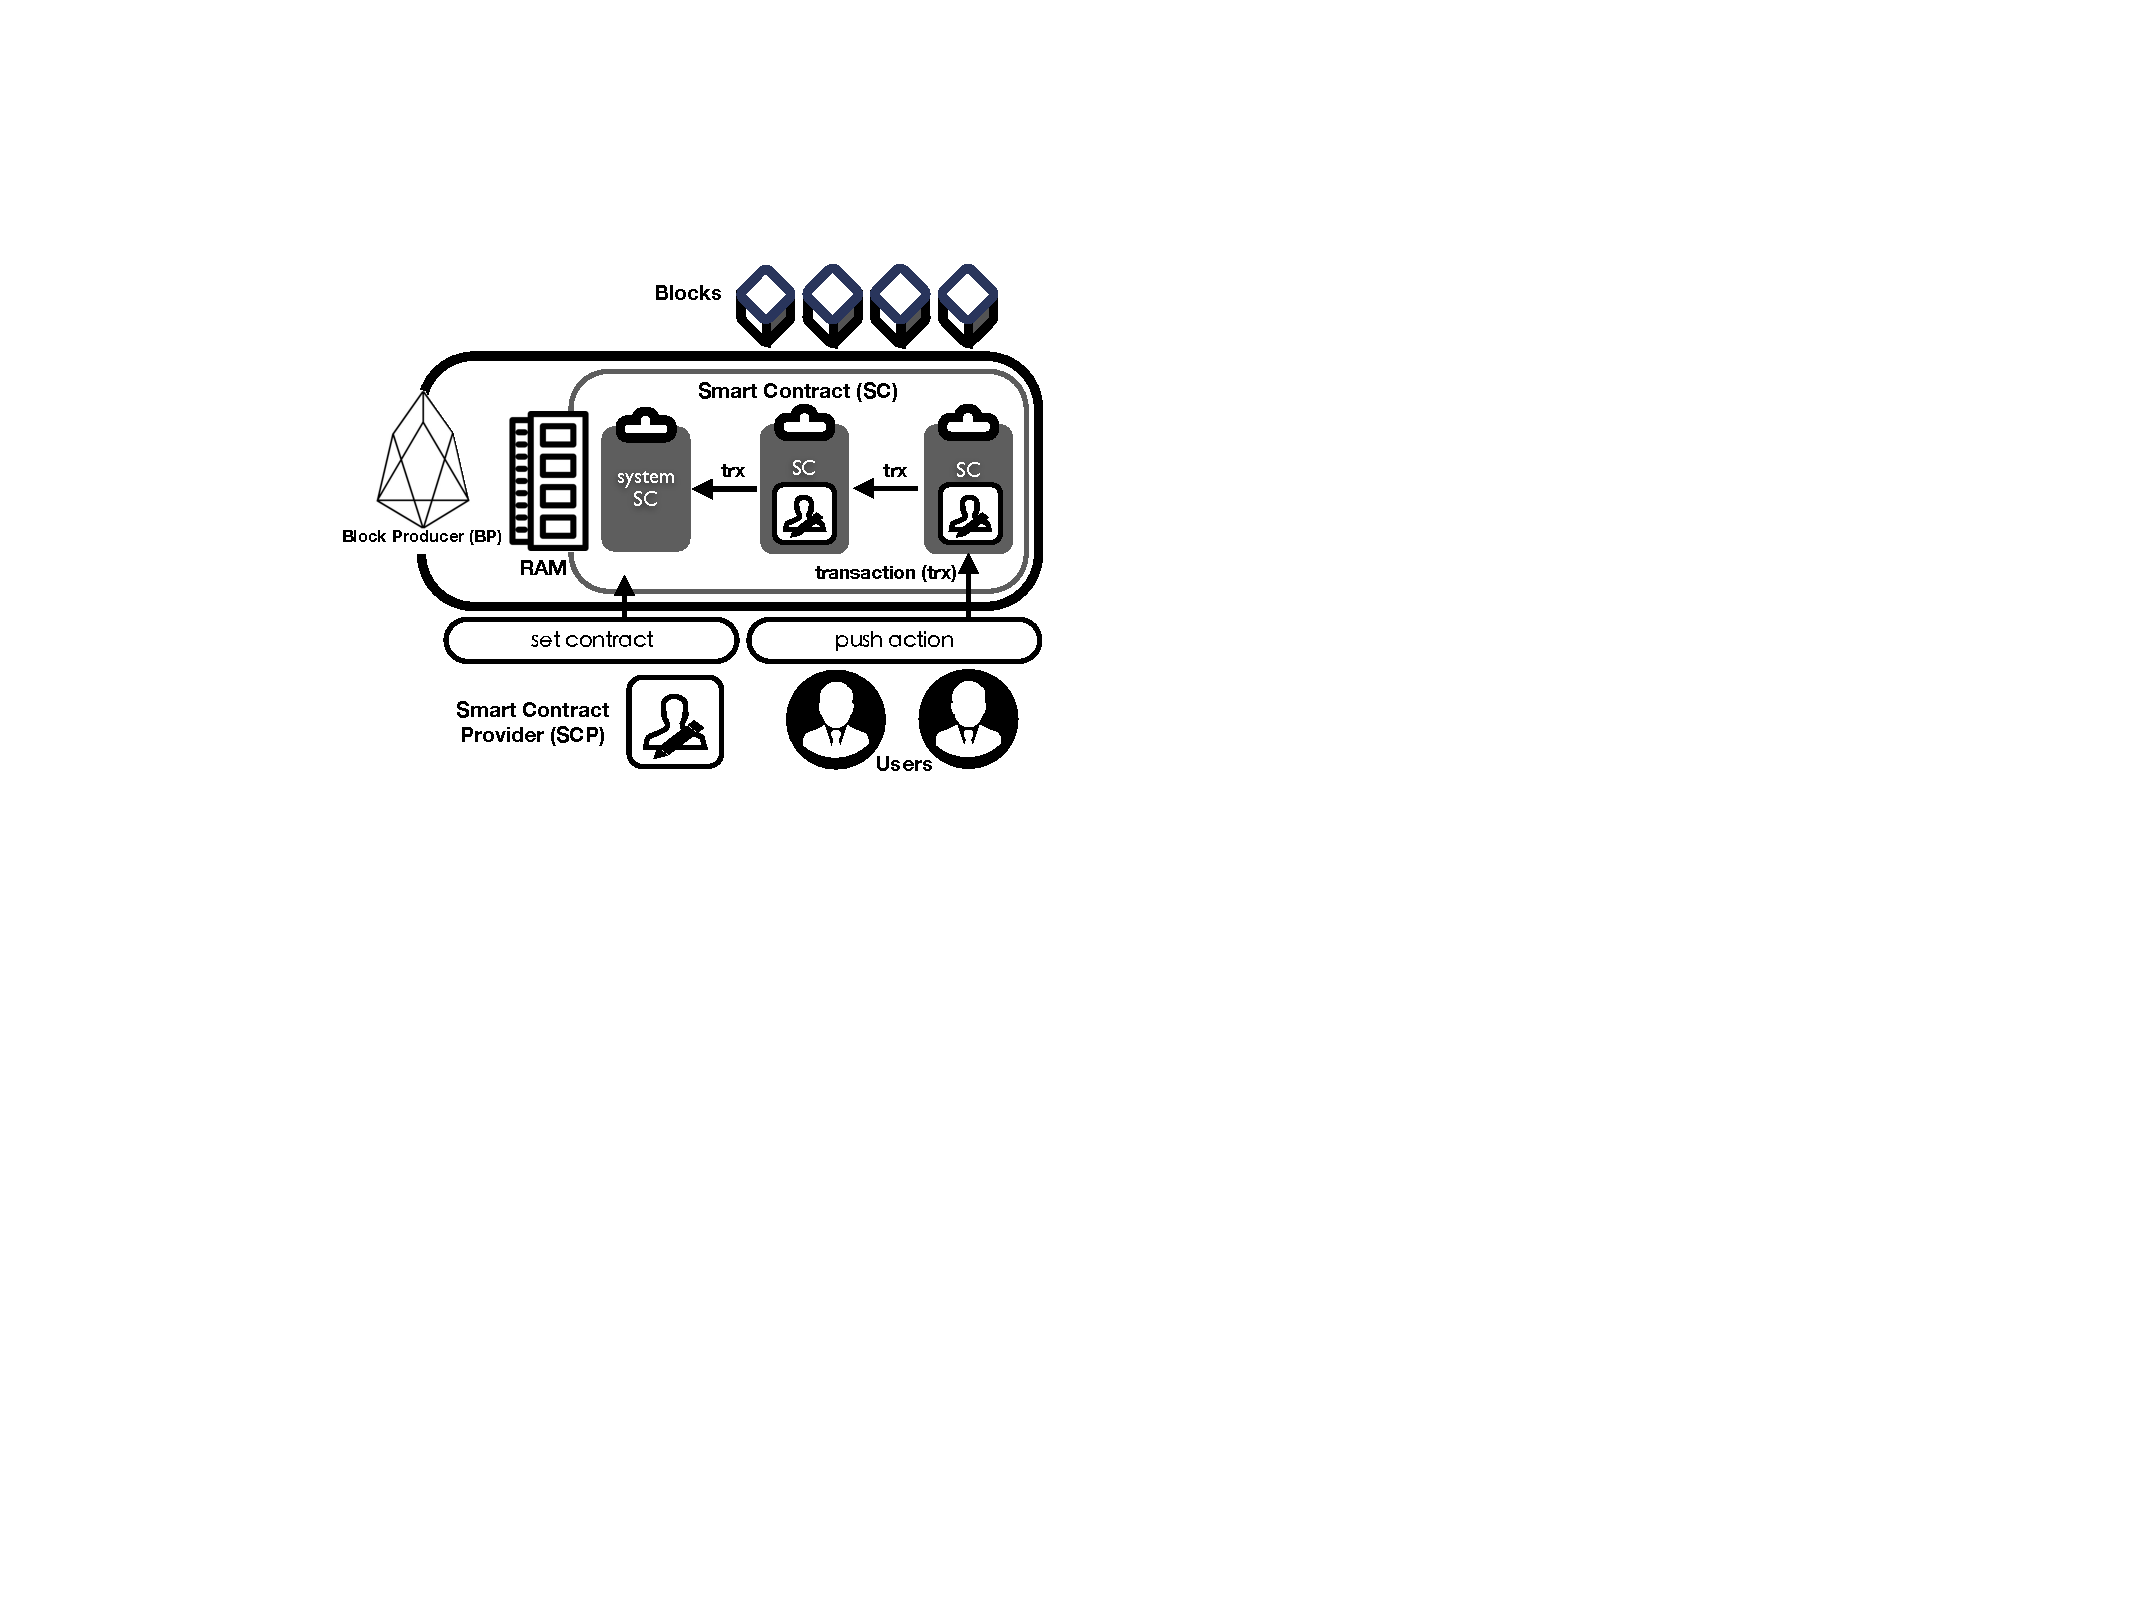
\includegraphics[width=\linewidth]{figures/philosophy.pdf}
  \caption{Architecture of \PLATFORM}
  \label{fig:overview}
\end{figure}

% What is EOS.
\eos is a blockchain system for a cryptocurrency called EOS. In this section, we
describe the main characteristics of \eos. As some parts of its
whitepaper~\cite{EOSWHITEPAPER} are outdated and ambiguous, we interpret them
based on our judgment by carefully analyzing the \eos source code.
%and referring this article~\cite{xueos}.
%
~\autoref{fig:overview} illustrates a simplified overview of the \eos ecosystem.
%
The main difference between \eos and the other blockchain systems lies in its
consensus algorithm, which is the core of the blockchain system.
%
Unlike the other blockchain systems of the top cryptocurrencies in the
market~\cite{coincap}, \eos adopted \textit{Delegated Proof of Stake
(DPoS)}~\cite{larimer2014delegated} as its consensus algorithm. DPoS delegates
the role of a node in a blockchain system to a small number of representative
nodes, known as \textit{Block Producers (\BPs)}.
%
Among the nodes in the \eos network, 21 BPs are selected through a voting
procedure; these BPs are responsible for deciding whether newly created blocks
can be attached to the current chain.
%
With DPoS, \eos is able to significantly speed up its transaction rate.

Another feature of \eos is its ability to execute a \textit{smart contract
(\SC)}, which is essentially a program developed by a user. It is similar to
those supported by the \eth platform~\cite{wood2014ethereum}. In this paper,
we call the developers of \SCs as \textit{Smart Contract Providers (\SCPs)}.
%
In the \eos system, if a user wants to execute an SC, s/he can send a
\textit{transaction} to one of the BPs in the \eos network.
%
This transaction consists of several \textit{actions} that specify a target
\SC and the parameters for the execution of the \SC.
%
%If the recipient node is not a BP, the transaction is finally transferred to
%one of the BPs.
When the \BP receives the transaction, it executes the requested \SC after
fetching the SC from the \eos chain and creates a new \eos block that stores
the execution results. Then, the new block is propagated to the other BPs
through a broadcasting procedure.



\section{\eos smart contract}
\label{ss:contract}
% 컨트랙트가 수정 가능한 배경 제시
An \SC often refers to a computer program that executes on a blockchain system
or a distributed ledger. Many blockchain ecosystems, including \eth and \eos,
support the execution of a given SC for various purposes, including banking,
gambling, initial coin offerings (ICOs), and trading in the marketplace~\cite{
dappradar}.

The design of \eth, the most popular blockchain system that supports \SCs,
demands that every \SC in their system should be unchangeable; thus, it allows
no revision not even for updating the source code or fixing vulnerabilities in
the \SCs. Therefore, \SCPs, in practice, dispose of their \SCs and create new
ones in order to patch inherent bugs.

On the other hand, \eos allows \SCPs to modify their \SCs. However, this design
decision entails another problem that \SCPs are able to change the semantics of
their \SCs, which are then executed by users without any active notification of
the change.
%
Therefore, users have few options but to completely trust \SCPs to execute their
\SCs while understanding that these \SCs may be changed at any time.

The option still remains for users to analyze an \SC to understand its semantics
before executing the \SC; however, \SCs in the \eos system are binary programs
compiled in the form of \textit{Web Assembly}~\cite{bastien2015webassembly},
which makes the understanding of their semantics difficult.
%
Furthermore, \SCPs are under no responsibility to open the source code of
their \SCs. According to one of the \eos explorers called EOS Park, only
10\% of \SCPs release their source code publicly~\cite{eospark}.
%
These characteristics of \eos make it difficult for users to analyze each \SC,
further contributing to users having no choice, but to trust the goodwill of \SCPs.



\section{Resources of \eos}
\label{ss:stake}

Every transaction and execution involving SCs in the \eos system consumes
resources.
%
By design, the system abstracts its resources into three items: computational
power, network bandwidth, and storage. For convenience, in this paper, we call
these as \cpu, \net, and \ram, respectively.
%
When a user directs a transaction to run an SC, the user should already have
enough resources for the consumption by the SC, called \textit{transaction costs}.
%
Therefore, the platform asks participating SCPs and users to purchase \ram or
to stake \cpu and \net.
%
Here, \emph{staking} refers to an action of allocating a certain number of EOS
tokens (i.e., EOS cryptocurrency) to reserve BP resources.

\eos adopted this mechanism to effectively manage the constrained resources of
the BPs and prevent resource abuse.
%
More specifically, when a user stakes EOS tokens, \eos distributes the capacity
of the resources to a user proportional to the tokens staked by this user.
%
For example, if a user staked 1\% of the total staked EOS tokens, then the user
is allowed to use 1\% of the total resource capacity as well.
%
Staked tokens do not disappear but are marked as staked in the system. That is,
a user can unstake his/her tokens anytime, and the tokens become available after
three days. At the time of unstaking, the staked \cpu and \net are also
released.
%
On the other hand, the tokens of the purchased \ram are not returned. \ram is 
storage for the data used within an SC, and the user can refund \ram only if the
data used in the target SC is removed.
%
Therefore, a user should consider using his/her resources wisely.





\section{\EOS resource payment}
\label{ss:receiver}

The underlying design philosophy for \eos is \emph{Receiver Pays}, denoting that
SCPs should pay for the usage of their SCs by users.
%
More specifically, a user only pays for the initial transaction cost, while the
SCP pays for the other costs of the subordinate transactions which come within
the first SC.
%
Consequently, the costs of running SCs become the business costs for which 
SCPs should be responsible. SCPs stake their \cpu and \net for the users who 
execute their SCs, and the amount of staked resources strongly affects the 
number of processed transactions from users.

However, it is burdensome for those SCPs who require a large amount of \cpu and
\net to execute their SCs. In such cases, SCPs can delegate the resource usage to
users.
%
Even though \eos enables the SCPs to delegate the transaction costs to the
users, it requires an additional permission, called the \code, from the users. If
this permission is given, an SCP can control all the resources of a user,
including EOS tokens.
%`
As a result, since most users would not want to give their permission to an
SCP, many SCPs follow the Receiver Pays model by paying for the business costs
during the execution of their SCs.
